\begin{center}\large\textbf{Readings: 12.1-12.6 pg 540 - 583}\\
\normalsize \end{center}
\large \hlinewd{2pt}
~\\\textbf{A general linear model:}\\
Models which can include both qualitative and/or quantitative explanatory variables are called general linear models or GLMs.  (Again, the `linearity' pertains to the parameters, not the explanatory variables.)\\~\\

\textbf{How to write qualitative variables in a GLM format?}\\~\\
\textbf{ANOVA (Analysis of Variance, i.e. comparing mean squares) revisited:}\label{ANOVAreview}\\~\\
The One-Way ANOVA model is used when we wish to compare the means of $t$ different groups.  (One-Way corresponds to having only one factor of interest.)\\~\\
Often a completely randomized experimental design will be analyzed using an ANOVA model.  \\~\\
One form of the One-Way ANOVA model is
$$Y_{ij}=\mu+\tau_i+E_{ij}$$
\begin{itemize}
\item $E_{ij}$ are i.i.d. $N(0,\sigma^2)$\
\item $i=1,...,t$ describes the treatment group
\item $j=1,...,n_i$ represents the number of observations we have in treatment group $i$. 
\end{itemize}
We will consider `balanced' designs for now, where $n_i=n$, same number of replicates for each treatment.  Total number of observations = $N = nt$\\~\\

\newpage

\textbf{Unknown parameters:}
\begin{itemize}
\item $\mu$ - overall population mean (avg of treatment population means)
\item $\tau_i$ - difference between (population) mean for treatment $i$ and $\mu$
\item $\sigma^2$ - (population) variance within a given treatment group (constant across groups)
\end{itemize}
~\\
\textbf{Goals of One-Way ANOVA}: Determine
\begin{enumerate}
\item if all treatment means are equal.
\item if treatment means not equal, which means differ from eachother.
\end{enumerate}
~\\

\textbf{One-Way ANOVA example}:\\
An experiment was done to determine if there was a difference between antibiotic types in terms of their binding fraction in bovines.  There were N=20 bovines that were randomly assigned to one of t=5 types of antibiotics (the levels of the factor, since only one factor these levels are also the treatments), yielding n=4 replicates for each treatment.  The data given here, labeled in terms of the One-Way ANOVA format:
\begin{center}
\begin{tabular}{lc|cc} 
Binding Fraction (Y) & Antibiotic& True Trt Mean & Sample Mean\\\hline
$Y_{11}=29.6$ & Penicillin G &\multirow{4}{*}{$\mu+\tau_1$}&\multirow{4}{*}{$\bar{y}_{1+}=28.6$}\\
$Y_{12}=24.3$ & Penicillin G \\
$Y_{13}=28.5$ & Penicillin G \\
$Y_{14}=32.0$ & Penicillin G \\\hline
$Y_{21}=27.3$ & Tetracyclin&\multirow{4}{*}{$\mu+\tau_2$}&\multirow{4}{*}{$\bar{y}_{2+}=31.4$}\\
$Y_{22}=32.6$ & Tetracyclin\\
$Y_{23}=30.8$ & Tetracyclin\\
$Y_{24}=34.8$ & Tetracyclin\\\hline
$Y_{31}=5.8$ & Streptomycin&\multirow{4}{*}{$\mu+\tau_3$}&\multirow{4}{*}{$\bar{y}_{3+}=7.8$}\\
$Y_{32}=6.2$ & Streptomycin\\
$Y_{33}=11.0$ & Streptomycin\\
$Y_{34}=8.3$ & Streptomycin\\\hline
$Y_{41}=21.6$ & Erythromycin&\multirow{4}{*}{$\mu+\tau_4$}&\multirow{4}{*}{$\bar{y}_{4+}=19.1$}\\
$Y_{42}=17.4$ & Erythromycin\\
$Y_{43}=18.3$ & Erythromycin\\
$Y_{44}=19.0$ & Erythromycin\\\hline
$Y_{51}=29.2$ & Chloramphenicol&\multirow{4}{*}{$\mu+\tau_5$}&\multirow{4}{*}{$\bar{y}_{5+}=27.8$}\\
$Y_{52}=32.8$ & Chloramphenicol\\
$Y_{53}=25.0$ & Chloramphenicol\\
$Y_{54}=24.2$ & Chloramphenicol\\\hline
\multicolumn{4}{l}{$\bar{y}_{++}=22.9$}\\
\end{tabular}
\end{center}

Goal: Test if the population means for these 5 treatments are plausibly equal. \\
If so, which treatment means differ significantly? \\~\\
\textbf{Modeling the binding fraction experiment:}\\
One-Way ANOVA model is appropriate: 
$$Y_{ij} = \mu + \tau_i + E_{ij}$$
for $i=1,\ldots,5$ and $j=1,\ldots,4$, where $E_{ij}$ are i.i.d. $N(0,\sigma^2)$ errors. \\~\\

To test $H_0: \tau_1 = \tau_2 = \ldots = \tau_5 =0$, we just carry out One-Way ANOVA table and look at global p-value.\\~\\
\textbf{Table for balanced one-way ANOVA:}
\begin{center}
\begin{tabular}{|c|c|c|c|c|} \hline
Source & DF & SS & MS & F \\ \hline
Treatments & $t-1$ & $SS(T)$ & $MS(T)=\frac{SS(T)}{(t-1)}$ & $F=\frac{MS(T)}{MS(E)}$ \\ 
Error & $t(n-1)$ & $SS(E)$ & $MS(E)=\frac{SS(E)}{(N-t)}$ & \\
Total & $nt-1$ & $SS(TOT)$ & &\\ \hline
\end{tabular}
\end{center}
where
\begin{eqnarray*}
SS(T) & = &\sum_{i=1}^{t} \sum_{j=1}^{n} (\bar{y}_{i+} - \bar{y}_{++})^2 = n\sum_{i=1}^{t}(\bar{y}_{i+} - \bar{y}_{++})^2\\
SS(E) & = & \sum_{i=1}^{t} \sum_{j=1}^{n}(y_{ij}-\bar{y}_{i+})^2 \\
SS(Tot)&=& \sum_{i=1}^{t} \sum_{j=1}^{n}(y_{ij}-\bar{y}_{++})^2
\end{eqnarray*}
Note:  SS(T) is also called SS(Between) and SS(E) is also called SS(Within).\\~\\

\newpage

For our example, 
\begin{center}
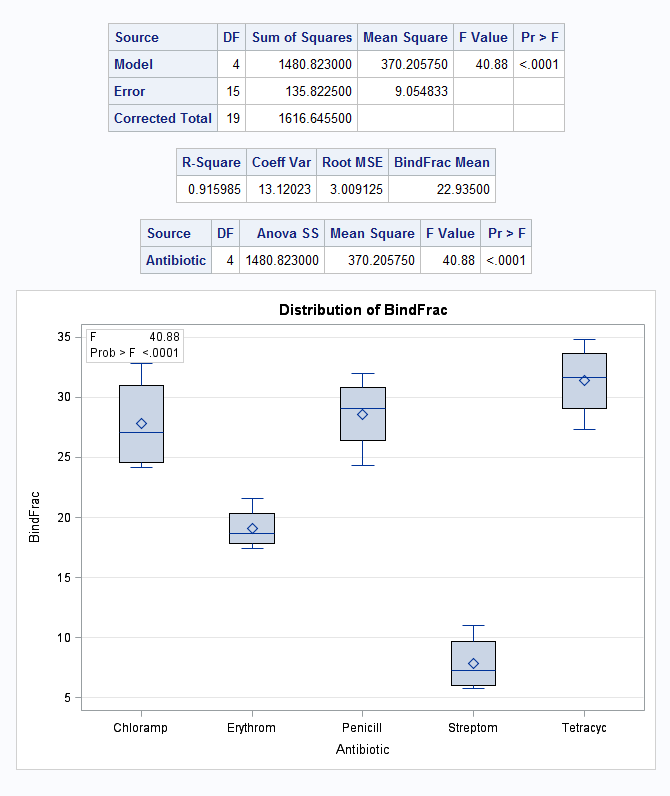
\includegraphics[scale=0.5]{BindFracANOVA}\includegraphics[scale=0.4]{BindFracBoxplot}
\end{center}

Conclusion about treatment means begin equal?\\~\\~\\

Parameter estimates:
\begin{itemize}
\item $\hat\mu = \bar{y}_{++}$
\item $\hat\tau_i = \bar{y}_{i+}-\bar{y}_{++}$ and standard errors of treatment means are $\sqrt{\frac{MS(E)}{n}}$
\item To compare treatment means we look at $\hat\tau_i-\hat\tau_j=\bar{y}_{i+}-\bar{y}_{j+}$ with SE $= \sqrt{\frac{2MS(E)}{n}}$
\end{itemize}

\newpage

\textbf{Matrix formulation of the GLM representation of the One-way ANOVA model: (will allow us to make inference just as we've done previously!)}\\~\\
\begin{center}
\begin{tabular}{ccc}
\textbf{y}=$\left(\begin{array}{c} 29.6\\24.3\\28.5\\32.0\\27.3\\32.6\\30.8\\34.8\\5.8\\6.2\\11.0\\8.3\\21.6\\17.4\\18.3\\19.0\\29.2\\32.8\\25.0\\24.2\\\end{array}\right)$ &
\textbf{X} = $\left(\begin{array}{ccccc}
1 & 1 & 0 & 0 & 0 \\
1 & 1 & 0 & 0 & 0 \\
1 & 1 & 0 & 0 & 0 \\
1 & 1 & 0 & 0 & 0 \\
1 & 0 & 1 & 0 & 0 \\
1 & 0 & 1 & 0 & 0 \\
1 & 0 & 1 & 0 & 0 \\
1 & 0 & 1 & 0 & 0 \\
1 & 0 & 0 & 1 & 0 \\
1 & 0 & 0 & 1 & 0 \\
1 & 0 & 0 & 1 & 0 \\
1 & 0 & 0 & 1 & 0 \\
1 & 0 & 0 & 0 & 1 \\
1 & 0 & 0 & 0 & 1 \\
1 & 0 & 0 & 0 & 1 \\
1 & 0 & 0 & 0 & 1 \\
1 & 0 & 0 & 0 & 0 \\
1 & 0 & 0 & 0 & 0 \\
1 & 0 & 0 & 0 & 0 \\
1 & 0 & 0 & 0 & 0
\end{array}\right)$ &
$\boldsymbol{\beta}$=$\left(\begin{array}{c} \beta_0 \\\beta_1\\\beta_2\\\beta_3\\\beta_4\\\end{array}\right)$ 
\end{tabular}
\end{center}

\newpage

SAS proc glm code and output are given below:\\
\begin{small}
\begin{verbatim}
proc glm data=binding;
class antibiotic;
model bindfrac=antibiotic/solution inverse;
run;
\end{verbatim}
\end{small}

\begin{center}
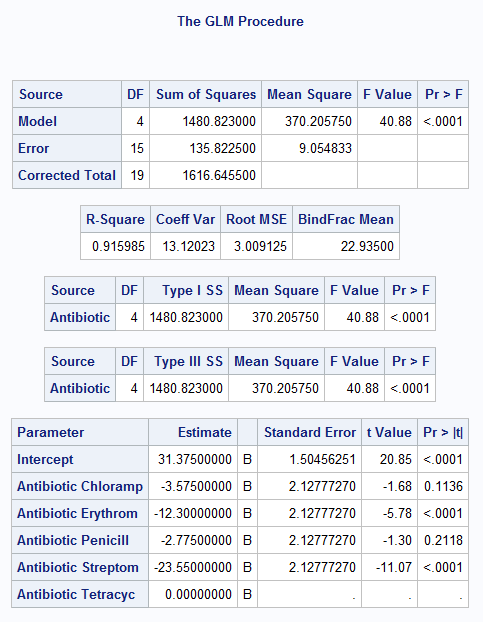
\includegraphics[scale=0.75]{BindFracGLM}\\
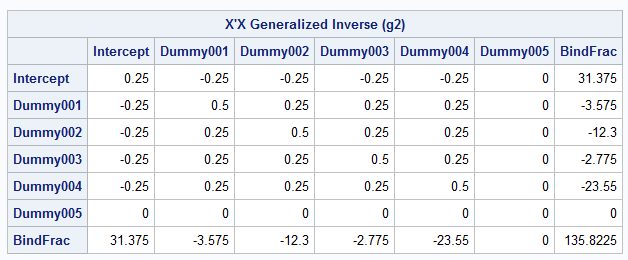
\includegraphics[scale=0.75]{BindFracGLMInverse}
\end{center}

\newpage

Estimates of the $\beta$'s still found by 
\[\hat{\boldsymbol{\beta}}= (\textbf{X}'\textbf{X})^{-1}\textbf{X}'\textbf{Y} = \left(\begin{array}{r} 27.8 \\ 0.8 \\ 3.6 \\
-20.0 \\ -8.7 \end{array} \right)
\]
Estimates for the five treatment means obtained by using combinations from the $\hat{\boldsymbol{\beta}}$ vector 
$$\mu(x_1,x_2,x_3,x_4)=\beta_0 + \beta_1 x_1 + \beta_2 x_2 + \beta_3 x_3 + \beta_4 x_4$$
$$\mbox{Trt 1 estimate} = \hat\mu(1,0,0,0) = \hat\beta_0 + \hat\beta_1 =  28.6 $$
$$\mbox{Trt 2 estimate} = \hat\mu(0,1,0,0) = \hat\beta_0 + \hat\beta_2 =  31.4 $$
$$\mbox{Trt 3 estimate} = \hat\mu(0,0,1,0) = \hat\beta_0 + \hat\beta_3 =  ~7.8 $$
$$\mbox{Trt 4 estimate} = \hat\mu(0,0,0,1) = \hat\beta_0 + \hat\beta_4 =  19.1 $$
$$\mbox{Trt 5 estimate} = \hat\mu(0,0,0,0) = \hat\beta_0~~~~~~~ =  27.8$$

For standard errors of the $\hat{\beta}$'s we still have our variance-covariance matrix $\hat{\boldsymbol{\Sigma}}=MS(E)(\textbf{X}^{T}\textbf{X})^{-1}$
\[ 
\hat{\boldsymbol{\Sigma}} = MS(E) (\textbf{X}'\textbf{X})^{-1} = \left(\begin{array}{rrrrr} 
2.3   & -2.3      & -2.3      & -2.3      & -2.3 \\
      & 4.5       & 2.3       & 2.3       & 2.3 \\
      &           & 4.5       & 2.3       & 2.3 \\
      &           &           & 4.5       & 2.3 \\
      &           &           &           & 4.5 \\
\end{array} \right)
\]

Note the pattern, what is the reason for it?\\~\\~\\~\\~\\~\\

To get SE's of our treatment mean estimates we can use vectors:  Let $\textbf{a},\textbf{b},\textbf{c},\textbf{d}$ be defined by 
$$\textbf{a}^{T}=(1,1,0,0,0), \textbf{b}^{T}=(1,0,1,0,0), \textbf{c}^{-1}=(1,0,0,1,0), \textbf{d}^{T}=(1,0,0,0,1).$$
Then
\[
\begin{array}{lclcl}
\hat\mu(1,0,0,0) & = & \hat\beta_0  + \hat\beta_1 & = & \textbf{a}^{T}\hat\beta \\
\hat\mu(0,1,0,0) & = & \hat\beta_0  + \hat\beta_2 & = & \textbf{b}^{T}\hat\beta \\
\hat\mu(0,0,1,0) & = & \hat\beta_0  + \hat\beta_3 & = & \textbf{c}^{T}\hat\beta \\
\hat\mu(0,0,0,1) & = & \hat\beta_0  + \hat\beta_4 & = & \textbf{d}^{T}\hat\beta \\
\hat\mu(0,0,0,0) & = & \hat\beta_0  & = & \hat\beta_0 
\end{array}
\]
and for a balanced design the variances are all the same and are given by
$$\textbf{a}' \hat{\boldsymbol{\Sigma}} \textbf{a} = \textbf{b}' \hat{\boldsymbol{\Sigma}} \textbf{b} = \textbf{c}' \hat{\boldsymbol{\Sigma}} \textbf{c} = \textbf{d}' \hat{\boldsymbol{\Sigma}} \textbf{d} = \widehat{\Var}(\hat\beta_0) = \widehat{\Var}(\hat\beta_0 + \hat\beta_j) = 2.3$$
so the estimated SE for any sample treatment mean is $\sqrt{2.3}=1.5$.\\~\\

Recall from one-way ANOVA that 
$$\widehat{SE}(\tmean{i}) = \sqrt{\frac{MS(E)}{n}} = \sqrt{\frac{9.1}{4}} = \sqrt{2.3} = 1.5$$
and that for differences between treatment means 
$$\widehat{SE}(\tmean{i}-\tmean{j})=\sqrt{\frac{2MS(E)}{n}}=\sqrt{4.5} = 2.1$$
~\\

\textbf{Now we have a framework to use both quantitative and categorical explanatory variables at the same time!}\\~\\
\textbf{A general linear model for 5k times of men AND women:}\\
Using $X_1$=Age, we fit a quadratic model $\mu(x_1) = \beta_0 + \beta_1 x_1 + \beta_1 x_1^2$ for to predict the mean pace for runners.  Consider modeling gender (a categorical variable) as well.\\
Let $x_3$ be defined by  
\[
x_3 = 
\begin{cases} 
1 & \text{female} \\ 0 & \text{male} 
\end{cases}
\]
Some candidate models:
\begin{enumerate}
\item The `null' model:
$$\mu(x_1,x_3) = \beta_0$$~\\
\item The One-Way ANOVA model in GLM form:
$$\mu(x_1,x_3) = \beta_0 + \beta_3 x_3$$~\\
\item The SLR model using Age:
$$\mu(x_1,x_3) = \beta_0 + \beta_1 x_1$$~\\
\item The MLR model quadratic in Age:
$$\mu(x_1,x_3) = \beta_0 + \beta_1 x_1+ \beta_2 x_1^2 $$~\\
\item A GLM that allows for different intercepts for our parabolas:  
$$\mu(x_1,x_3) = \beta_0 + \beta_1 x_1+ \beta_2 x_1^2+ \beta_3 x_3  $$
This model has intercept $\beta_0$ for males ($x_3=0$) and intercept $\beta_0+\beta_3$ for females ($x_3=1$).
$$\mbox{Equation for males: } \beta_0+\beta_1x_1+\beta_2x_1^2$$
$$\mbox{Equation for females: } (\beta_0+\beta_3)+\beta_1x_1+\beta_2x_1^2$$~\\
\item A GLM that allows for different intercepts and for different shapes of the parabolas:   
$$\mu(x_1,x_3) = \beta_0 + \beta_1 x_1+ \beta_2 x_1^2+ \beta_3 x_3 + \beta_4 x_1x_3 + \beta_5x_1^2x_3 $$
Intercepts as in the previous model.  `Linear' term for males is $\beta_1$ and is $\beta_1+\beta_4$ for females.  `Quadratic' term for males is $\beta_2$ and is $\beta_2+\beta_5$ for females. 
$$\mbox{Equation for males: } \beta_0+\beta_1x_1+\beta_2x_1^2$$
$$\mbox{Equation for females: } (\beta_0+\beta_3)+(\beta_1+\beta_4)x_1+(\beta_2+\beta_5)x_1^2$$~\\
\end{enumerate}

We can fit these models in proc glm using the following code: (Note: each model must be done in a separate proc glm statement)
\begin{small}
\begin{verbatim}
proc glm;
class sex;
title 'Model 2';
model pace=sex;
title 'Model 3';
model pace=age;
title 'Model 4';
model pace=age age*age;
title 'Model 5';
model pace=age age*age sex;
title 'Model 6';
model pace=age age*age sex sex*age sex*age*age;
run;
\end{verbatim}
\end{small}


\begin{center}
\includegraphics[scale=0.8,page=2,trim=5mm 85mm 5mm 5mm]{ResRunGLM.pdf}
\includegraphics[scale=0.7,trim= 5mm 100mm 5mm 5mm,page=3]{ResRunGLM.pdf}
\includegraphics[scale=0.8,page=5,trim=5mm 100mm 5mm 15mm]{ResRunGLM.pdf}
\includegraphics[scale=0.8,trim= 5mm 150mm 5mm 5mm,page=6]{ResRunGLM.pdf}
\includegraphics[scale=0.8,page=8,trim=5mm 85mm 5mm 5mm]{ResRunGLM.pdf}
\includegraphics[scale=0.8,trim= 5mm 150mm 5mm 5mm,page=9]{ResRunGLM.pdf}
\includegraphics[scale=0.8,page=11,trim=5mm 85mm 5mm 5mm]{ResRunGLM.pdf}
\includegraphics[scale=0.8,trim= 5mm 150mm 5mm 5mm,page=12]{ResRunGLM.pdf}
\includegraphics[scale=0.8,page=14,trim=5mm 85mm 5mm 5mm]{ResRunGLM.pdf}
\includegraphics[scale=0.8,trim= 5mm 5mm 5mm 5mm,page=15]{ResRunGLM.pdf}
\end{center}

\newpage

\textbf{Analysis of covariance, ANCOVA or ACOVA:}\\
Recall the three principles of experimental design:
\begin{itemize}
\item Randomization
\item Replication
\item Error Reducing Methods
\end{itemize}

One method of error reduction we looked at was blocking.  Here we split up the EUs and then randomize treatments to each block.  In this way, every treatment occurs in each block and the block effects cancel out.\\~\\
We are not always able to block, sometimes we don't have the value of the covariate until after the experiment is done.  A similar method that will account for these types of covariates is called Analysis of CoVariance (ANCOVA).\\~\\
Associations between covariates $z$ and the main response variable of interest $y$ can be used to reduce unexplained variation $\sigma^2$.\\~\\

\textbf{An nutrition example:}\\
A nutrition scientist conducted an experiment to evaluate the effects of four vitamin supplements on the weight gain of laboratory animals.  The experiment was conducted in a completely randomized design with $N=20$ animals randomized to $a=4$ supplement groups, each with sample size $n\equiv 5$.  The response variable of interest is weight gain, but calorie intake $z$ was measured concomitantly as couldn't separate EUs by this at the beginning.  

\begin{center}
\begin{tabular}{|cc|cc|cc|cc|} \hline
Diet & $y(g)$ & Diet & $y$ &Diet & $y$ &Diet & $y$ \\ \hline
1 & 48 & 2 & 65 & 3 & 79 & 4 & 59 \\
1 & 67 & 2 & 49 & 3 & 52 & 4 & 50 \\
1 & 78 & 2 & 37 & 3 & 63 & 4 & 59 \\
1 & 69 & 2 & 75 & 3 & 65 & 4 & 42 \\
1 & 53 & 2 & 63 & 3 & 67 & 4 & 34 \\ \hline
1 & $\tmean{1}=63.0$ & 2 & $\tmean{2}=57.4$  & 3 & $\tmean{3}=65.2$  & 4 & $\tmean{4}=48.8$ \\
1 & $s_1=12.3$ & 2 & $s_2=14.3$  & 3 & $s_3=9.7$  & 4 & $s_4=10.9$ \\ \hline
\end{tabular} 
\end{center}

Q: Is there evidence of a vitamin supplement effect?
\begin{center}
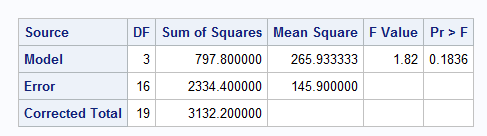
\includegraphics{DietsANOVA}
\end{center}
 
P-value $<$ 0.05, fail to reject $H_0$.  There is no evidence of a diet effect.\\~\\
Calorie intake $z$ was measured concomitantly:
\begin{center}
\begin{tabular}{ccc|ccc|ccc|ccc}
Diet & $y$ & $z\ \ $ & Diet & $y$ & $z\ \ $ &Diet & $y$ & $z\ \ $ &Diet & $y$ & $z\ \ $ \\ \hline
1 & 48 & 350 & 2 & 65 & 400 & 3 & 79 & 510 & 4 & 59 & 530 \\
1 & 67 & 440 & 2 & 49 & 450 & 3 & 52 & 410 & 4 & 50 & 520 \\
1 & 78 & 440 & 2 & 37 & 370 & 3 & 63 & 470 & 4 & 59 & 520 \\
1 & 69 & 510 & 2 & 73 & 530 & 3 & 65 & 470 & 4 & 42 & 510 \\
1 & 53 & 470 & 2 & 63 & 420 & 3 & 67 & 480 & 4 & 34 & 430 \\ \hline
\end{tabular} 
\end{center}

Q: How and why could these new data be incorporated into analysis? \\
A: A GLM can take into account both types of variables!  The method of ANCOVA can be used to reduce unexplained variation. \\
$$ Y_i = \beta_0 + \beta_1 x_{i1} + \beta_2 x_{i2} + \beta_3 x_{i3} + \beta_z z_i + E_i \ \ \mbox{ for }i=1,\ldots,20$$
where $x_{ij}$ is an indicator variable for subject $i$ receiving vitamin supplement $j$:
$$ x_{ij}=\begin{cases} 1 & \text{subject $i$ receives supplement $j$} \\  
0 & \text{else} \end{cases}$$
and errors $E_i \iid N(0,\sigma^2)$.\\~\\
Which Diet is being used as the baseline?\\
\textcolor{red}{Diet 4}\\~\\

Proceeding with MLR analysis of this GLM:

\begin{small}
\begin{verbatim}
proc glm data=diets;
class diet;
model gain = diet caloric;
run;
\end{verbatim}
\end{small}

\begin{center}
\includegraphics[page=2,scale=0.8,trim = 5mm 120mm 5mm 20mm]{DietsANCOVA}
\includegraphics[page=3,scale=0.6,trim = 5mm 150mm 5mm 5mm]{DietsANCOVA}
\end{center}

\newpage

\textbf{How can we estimate the mean weight gains for diet, taking into account the caloric intake?}\\
\textbf{Adjusted vs unadjusted means:}\\
The sample mean weight gains for the four diets and for the caloric intake for each diet group were
\begin{center}
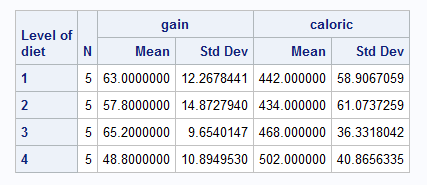
\includegraphics{DietsMeans}
\end{center}

The means for each diet are `unadjusted' means.  According to our analysis, caloric intake has a significant effect on weight gain.  However, each diet group had a different mean amount of caloric intake.  What does this imply?\\~\\~\\~\\~\\

Unadjusted means do not make any adjustment for the facts that 
\begin{enumerate}
\item caloric intake may vary by diet (presumably by chance, not because of diet)
\item weight gain depends on caloric intake
\end{enumerate}
~\\~\\
\textbf{Adjusted means} or \textbf{lsmeans} (least squares means) will estimate mean weight gains at a common value of our caloric intake (our covariate $z$).  The value often used for comparison is $\bar{z}$, the sample mean of the covariate.\\~\\

Here, $\bar{z}= (442+434+468+502)/4 = 461.5$.  The adjusted means are then just (the sub $a$ is to differentiate unadjusted means and adjusted means)
\begin{eqnarray*}
\bar{y}_{1,a} & = & \hat\beta_0 + \hat\beta_1 + \hat\beta_z (461.5) \\
\bar{y}_{2,a} & = & \hat\beta_0 + \hat\beta_2 + \hat\beta_z (461.5) \\
\bar{y}_{3,a} & = & \hat\beta_0 + \hat\beta_3 + \hat\beta_z (461.5) \\
\bar{y}_{4,a} & = & \hat\beta_0 + \hat\beta_z (461.5)
\end{eqnarray*} 

\newpage

To get SAS to report the estimated regression parameter vector $\hat{\boldsymbol{\beta}}$, use the {\tt solution} option in the model statement.  The default parametrization is the one we've adopted here where $\beta_0$ is the mean of the last level of the classification treatment factor:

\begin{center}
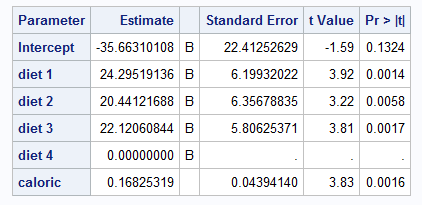
\includegraphics{DietsEstimates}
\end{center}

Substitution of $\hat{\boldsymbol{\beta}}$ into the expressions for adjusted means yields
\begin{eqnarray*}
\bar{y}_{1,a} & = & -35.7 + 24.3 + 0.17 (461.5) = 66.3\\
\bar{y}_{2,a} & = & -35.7 + 20.4 + 0.17 (461.5) = 62.4 \\
\bar{y}_{3,a} & = & -35.7 + 22.1 + 0.17 (461.5) = 64.1 \\
\bar{y}_{4,a} & = & -35.7 + + 0.17 (461.5) = 42.0 
\end{eqnarray*} 

These means are better for comparisons between diets as the effect of caloric intake (which affects weight gain) is constant across all the diets.  Thus, we are removing its effect.\\~\\

\newpage

To get proc glm to produce the estimates (above), unadjusted means (above), $(\textbf{X}^{T}\textbf{X})^{-1}$ matrix (below), adjusted means with standard errors (below), and CI's (below):

\begin{small}
\begin{verbatim}
proc glm data=diets;
class diet;
model gain = diet caloric/solution inverse;
means diet;
lsmeans diet/stderr cl;
run;
\end{verbatim}
\end{small}

\begin{center}
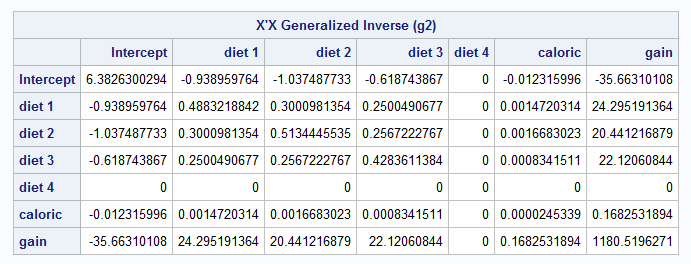
\includegraphics{DietsInverse}
\end{center}

The $(\textbf{X}^{T}\textbf{X})^{-1}$ matrix is found by removing the row/column with 0's and ignoring the row/column for the response.

\begin{center}
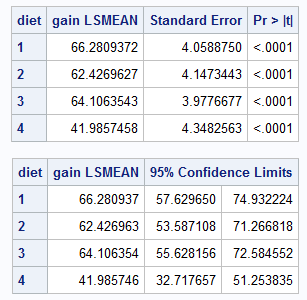
\includegraphics{DietsLSMeans}
\end{center}

We can now look at all pairwise differences of the lsmeans to see which levels differ significantly.\\~\\

\textbf{ANCOVA - What did we just do?  We used our covariate to reduce the unexplained variation in our response, allowing a clearer picture of our treatment differences. } \\~\\

\textbf{Huge assumptions of ANCOVA} - We assume the treatment \textit{does not} affect the covariate.  In this example, we assume the diets are not causing the animals to have different caloric intake (i.e. do not cause them to eat more or less). (We also need to do our usual assumption checking.)\\~\\
 We can inspect this assumption.  Let our covariate be our response and conduct an ANOVA using the diets as our treatments.  The global p-value will test if the caloric intake means differ significantly for each diet.  We hope to see no significance here!

\begin{small}
\begin{verbatim}
proc anova data=diets;
class diet;
model caloric = diet;
run;
\end{verbatim}
\end{small}

\begin{center}
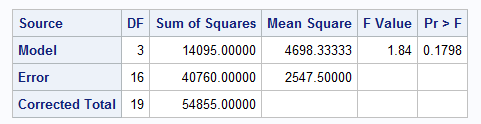
\includegraphics{DietsCaloricANOVA}
\end{center}

No evidence that treatment affects covariate.\\~\\




